\section{Manual}


\section{Step 1 - Installation}

\begin{itemize}
	\item Download the project provided at: https://github.com/CIoann/rabbit-eclipse.git
	\item Create a new workspace and import the project into Eclipse IDE
\end{itemize}

\section{Step 2 - Initialization} 
Before beginning the task you will need to run the environment to do that see figure (\ref{fig:rc})

\begin{figure}[!ht]
		\begin{center}		 	
			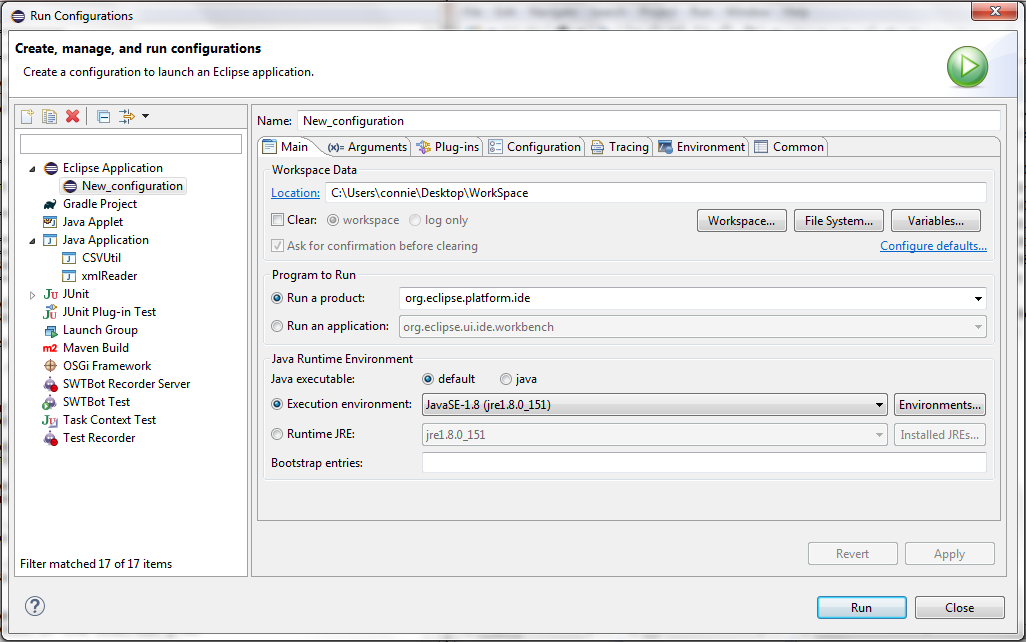
\includegraphics[width=\textwidth]{figures/runconfig.png}
		\end{center}
		\caption{Run Configuration.}
		\label{fig:rc}
	\end{figure}

Further you need to establish the plugin Rabbit, in order to do that you need to follow the steps presented below in figure \ref{fig:ir1} Select Window > Show View > Other > and then find Rabbit

\begin{figure}[!ht]
		\begin{center}		 	
			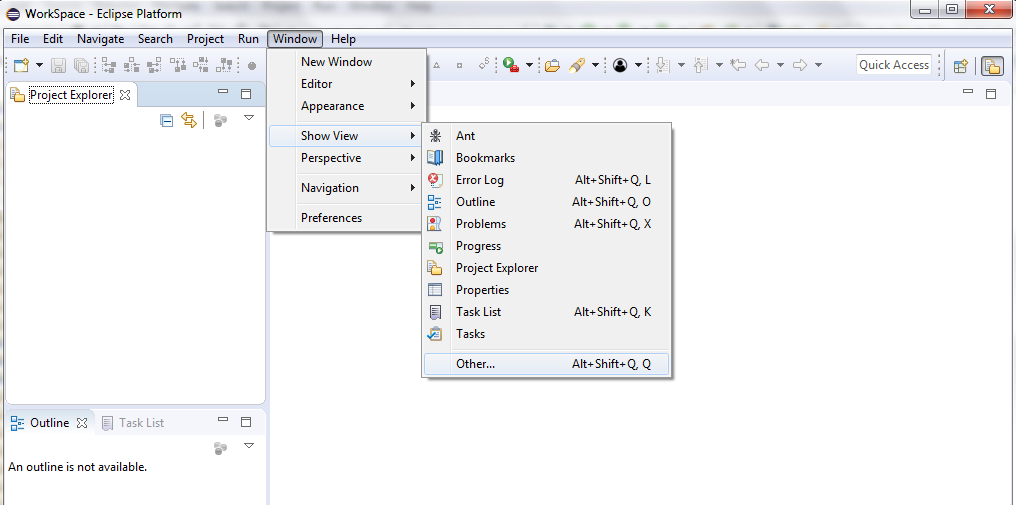
\includegraphics[width=\textwidth]{figures/ws1.png}
		\end{center}
		\caption{Initialise Rabbit}
		\label{fig:ir1}
	\end{figure}

At this point you are ready to continue.

\section{Step 3 - Your task}
The task is fairly simple, the purpose is the implementation of inheritance hierarchy of classes derive from an abstract superclass. Naming of methods and classes is important therefore is expected that you follow the provided notations (see Figure: \ref{cti}).

DessertShop class contains the functions of the shop as well as the test for your classes. Further you will need to implement:
\begin{itemize}
	\item DessertItem abstract superclass
	\item Candy, Cookie, IceCream classes which derive from DessertItem class
	\item Sundae class which derives from IceCream class
\end{itemize}

\textbf{The Candy class} should be derived from the DessertItem class. A Candy item has a weight and a price per pound which are used to determine its cost. For example, 2.30 lbs.of fudge @ .89 /lb. = 205 cents. The cost should be rounded to the nearest cent.

\textbf{The Cookie class} should be derived from the DessertItem class. A Cookie item has a number and a price per dozen which are used to determine its cost. For example, 4 cookies @ 399 cents /dz. = 133 cents. The cost should be rounded to the nearest cent.

\textbf{The IceCream class} should be derived from the DessertItem class. An IceCream item simply has a cost.

\textbf{The Sundae class} should be derived from the IceCream class. The cost of a Sundae is the cost of the IceCream plus
the cost of the topping.

	\begin{figure}[!ht]
		\begin{center}
		 	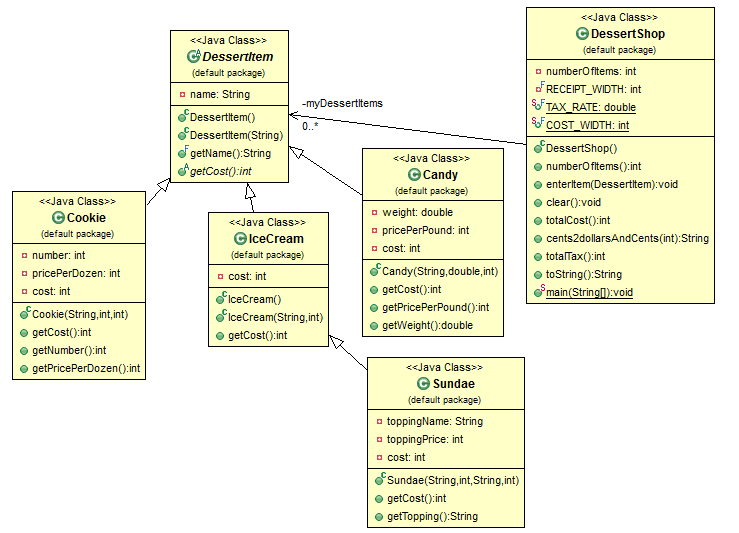
\includegraphics[width=\textwidth]{figures/cti.png}
 
		\end{center}
		\caption{Class Hierarchy.}
		\label{fig:cti}
	\end{figure}

\section{Step 4}








